\documentclass{article}

\usepackage{siunitx}
\usepackage{graphicx}
\usepackage{systeme}
\usepackage{amsmath}
\usepackage[ash]{realhats}
\usepackage{amsmath}
\graphicspath{ {./} }

\author{Emanuele Casciaro}
\title{Algoritmi per grafi}


\begin{document}
\maketitle
\tableofcontents

\newpage

\section{Introduzione}
In questo articolo verranno presentati degli algoritmi per grafi, in particolare la Depth First Search e l'implementazione di Prim dello Strongly Connected Component, valutandone le prestazioni in base all'estensione del grafo.

\section{Cenni teorici}
Vediamo adesso qualche definizione sui grafi.

\subsection{Grafo}
Un grafo può essere definito come un insieme di vertivi e di archi $G = (V, E)$, dove $V$ è l'insieme dei vertici $E$ è l'insieme degli archi, ossia di coppie di vertici. Ad ogni nodo $A$ e $B$, se collegati da un nodo $\exists (A, B) \in E$.
\newline
Un grafo è detto \textit{orientato} se la direzione degli archi è rilevante, pertanto se non lo è $(A, B) \in E \Rightarrow (B, A) \in E$.
Un gruppo di \textit{Strongly Connected Component} è un insieme di vertici tale che per ogni coppia di vertici esiste un percorso che li collega.
$$ \forall v_i, v_j \in S \subseteq V \exists v_i \rightarrow v_j $$

\section{Depth First Search}
È un algoritmo di esplorazione dei grafi, che consente di visitare ogni nodo del grafo, restituendo inoltre le informazioni circa i tempi di inizio e fine esplorazione di ogni nodo. L'algoritmo assegna ad ogni nodo tre colori:
\begin{itemize}
	\item \textbf{Bianco} per i nodi ancora non esplorati
	\item \textbf{Grigio} per i nodi la quale espolrazione è ancora in corso
	\item \textbf{Nero} per i nodi già esplorati
\end{itemize}
Occorre però chiarificare cosa significa per un nodo essere \textbf{grigio}: esplorare un nodo vuol dire esploarare tutti i suoi figli; allora un nodo diventerà grigio nel momento in cui inizierà la sua esplorazione, e diventerà nero una volta che non avrà più figli da esplorare.
Ciò allora ci da un criterio di arresto dell'esplorazione: si parte da un nodo detto \textit{radice} arbitrario e si inizia ad esplorare in modo ricorsivo i suoi figli, interrompendo ogni volta che si incontra un nodo non bianco.
\subsection{Tempi di esplorazioni}
Come detto in precedenza, l'algoritmo assegna ad ogni nodo i tempi di inizio e fine espolrazione, usate successivamente. Per com'è fatto l'algoritmo, è garantita la seguente proprietà. \newline
Per ogni coppia di vertici $v_i, v_j$, i tempi di inizio e fine esplorazione non si incrociano, ossia solo una delle seguenti è vera:
\begin{itemize}
	\item $[v_i.begin, v_i.end] \cap [v_j.begin, v_j.end] = [v_i.begin, v_i.end]$
	\item $[v_i.begin, v_i.end] \cap [v_j.begin, v_j.end] = [v_j.begin, v_j.end]$
	\item $[v_i.begin, v_i.end] \cap [v_j.begin, v_j.end] = \emptyset$
\end{itemize}
Questo teorema, detto teorema delle parentesi, è un risultato fondamentale che ci permetterà di formulare un algoritmo per il calcolo delle \textit{Strongly Connected Component}

\newpage
\section{Strongly Connected Component}

L'algoritmo si basa sul fatto che sia un grafo $G$ che la sua trasposta $G'$ condividono le stesse \emph{SCC}, cosa di cui ci si può convincere abbastanza facilemente osservando l'esempio sottostante.

\begin{figure}[h]
	\centering
	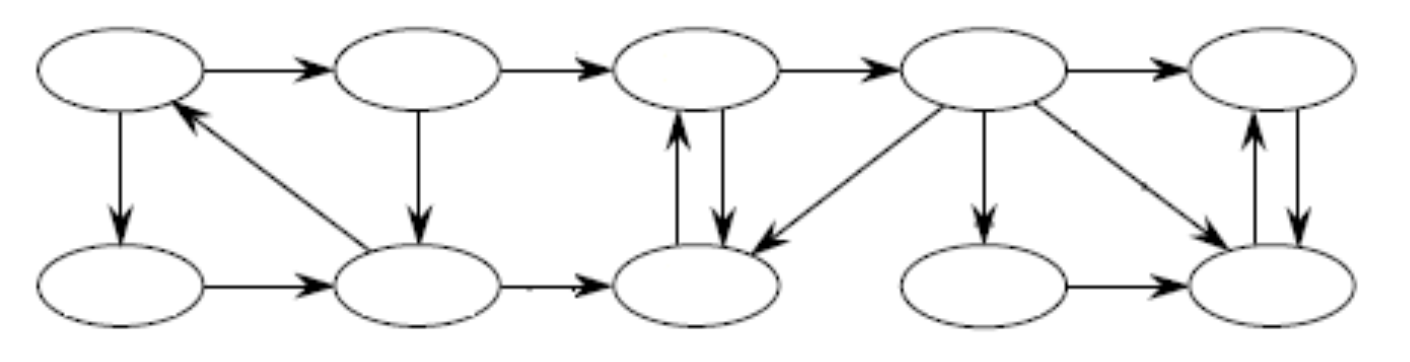
\includegraphics[width=1\linewidth]
	{"./graph1.png"}
	\label{graph}
\end{figure}

\begin{figure}[h]
\centering
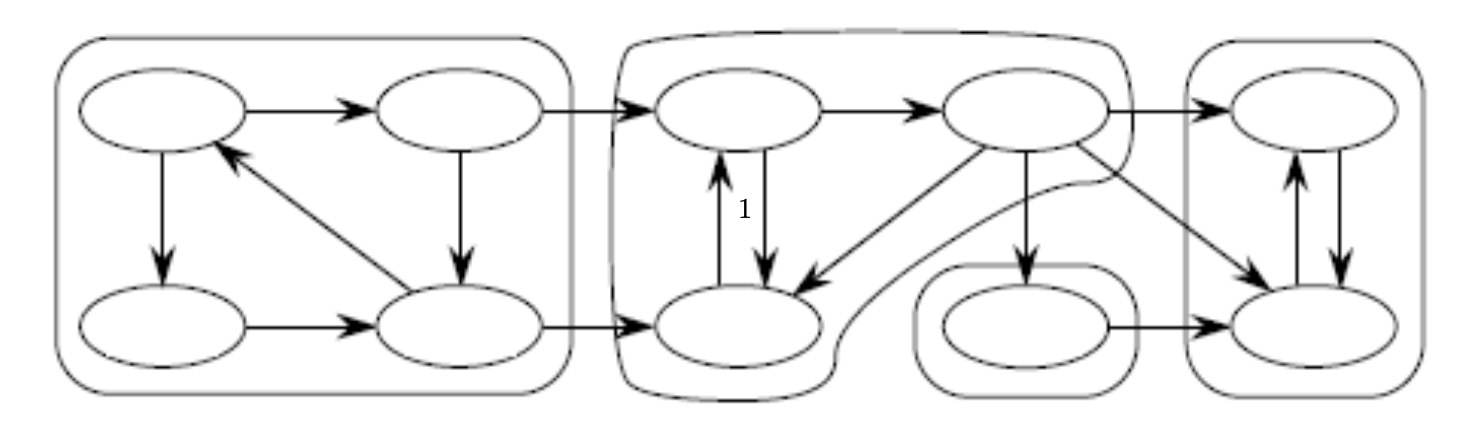
\includegraphics[width=1\linewidth]
{"./graph2.png"}
\label{graph}
\end{figure}

\begin{figure}[h]
\centering
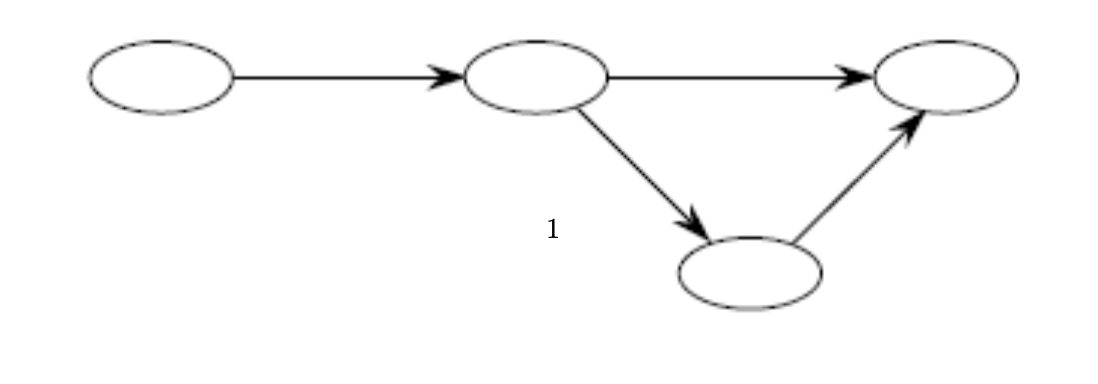
\includegraphics[width=1\linewidth]
{"./graph3.png"}
\label{graph}
\end{figure}
 In particolare, anche $G^{SCC} = (V^{SCC}, E^{SCC})$ è un grafo orientato.
 \subsection{Algoritmo}
 \begin{enumerate}
 	\item Calcola $DFS(G)$ per ottenere $v.f \forall v 	\in V$
 	\item Calcola $G^T$
 	\item Calcola $DFS(G^T)$ considerando in ordine decrescente rispetto a $u.f$
 	\item Genera l'output ad ogni iterazione come un singolo nodo contenente ogni nodo esplorato durente l'iterazione
 \end{enumerate}
Chiamando $DFS(G^T)$ con questo ordine si ha infatti che ad ogni iterazione possono essere esplorati soltanto i nodi appartententi all'SCC locale, oltre che a i nodi già esplorati, che verranno quindi ignorati. Ciò è appunto garantito in quanro considerando che il nodo a $v.f$ più alto nel grafo $G$ ha intuitivamente pochi figli in $G^T$, perchè avendo molti figli nel grafo di partenza, invertendo gli archi ne ha sicuramente pochi. E dato che le SCC sono le stesse a quell'iterazione esplorerà tutti e soli i nodi di tale SCC (non può uscire, in quanto gli archi sono invertiti).All'iterazione successiva, si inizierà da un nodo all'interno del SCC collegata a quella appena esplorata, e così via.
A questo punto non resta che raccogliere i nodi esplorati ad ogni iterazione e unirli in un unico nodo, mantenendo gli archi verso le altre SCC.
\section{Minimum Spanning Tree}
Dato un grafo non orientato pesato,  l'albero di connessione minima è l'albero che collega tutti i nodi nel modo più efficiente possibile. \newline Si ha quindi un peso $w(u, v) \forall (u, v) \in E$, che permette di formalizzare il problema in questo modo: 

Trovare $T^{*} \subseteq E$,  con $ T^{*} = arg$ $\underset{T}{min}$ $w(T) = \underset{(u, v) \in T}{\Sigma} w(u, v)$
\newline
Qualche definizione utile:
\begin{itemize}
	\item un \emph{taglio di V} $(V_A, V_S)$ è una partizione di $V$ di insieme disgiunti $V_A$ e $V_S$
	\item un \emph{arco} $(u, v) \in E$ \emph{attraversa} un taglio se $u \in V_A$ e $v \in V_S$ (o viceversa)
	\item un arco è \emph{leggero} per un taglio se ha \emph{peso minimo} rispetto a tutti gli archi che attraversano il taglio
\end{itemize}
Intuitivamente costruire un albero di soli archi leggeri porta ad avere un MST.
\newpage
\section{Algoritmo di Prim}
Costruisce l'MST a partire da un nodo casuale, aggiungendo ad ogni iterazione un \emph{arco sicuro} all'albero, fino a raggiungere tutti i nodi.
Per fare ciò si usa la struttura dati della coda di priorità, dove ogni nodo è ordinato (in modo crescente) in base al suo costo, definito come il peso minimo degli archi che lo collegano al sottoalbero $V_A$: così facendo il pop dalla coda si prende sempre un arco sicuro.

\begin{figure}[!h]
\centering
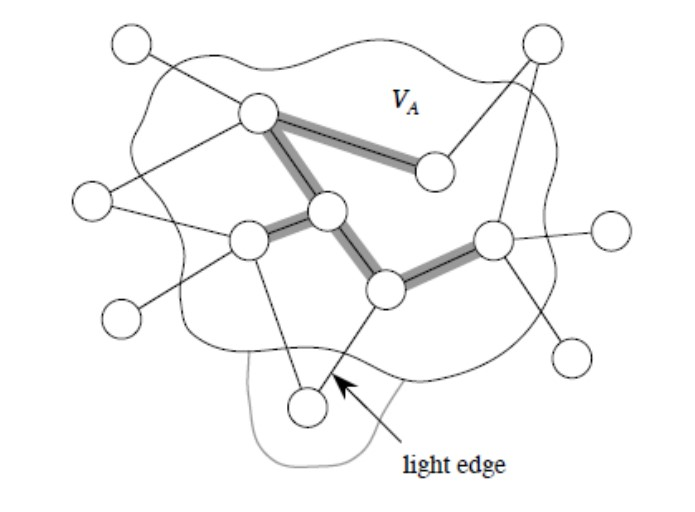
\includegraphics[width=0.7\linewidth]
{"./prim_example.jpg"}
\label{graph}
\end{figure}

\section{Test}
Ci sono due test principali: il primo testa l'algoritmo di Prim generando un grafo \emph{non orientato}, assegnando agli archi pesi casuali, per poi cercarne l'MST.\newline
Il secondo test invece riguarda la ricerca delle componenti fortemente connesse, in particolare si cerca una possibile relazione tra dimensione di un grafo e il suo numero di SCC: vengono creati una serie di grafi orientati, nei quali gli archi sono collocati in modo casuale, e si calcolano le loro SCCs, per ogni dimensione di grafo vengono calcolate le SCCs di più grafi, raccogliendone i dati sulla loro presenza, riportati poi in un grafico.
\section{Risultati attesi}
Data la casualità nell'assegnazione degli archi, mi aspetto che ci sia una relazione di proporzionalità diretta tra dimensione del grafo ed il suo numero di SCCs.
\newpage
\section{Risultati e conclusioni}
\subsection{Prim}
L'algoritmo di Prim ha dimostrato di poter generare un MST: a seguire un esempio della sua esecuzione
\begin{figure}[h]
\centering
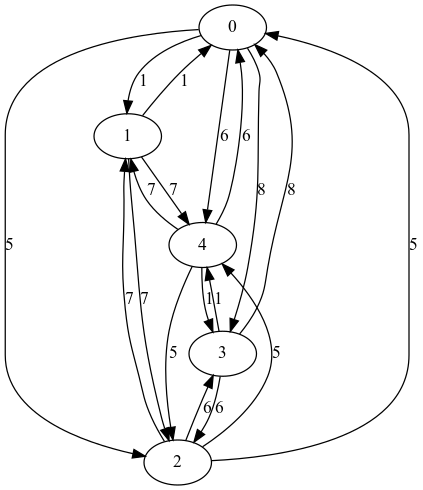
\includegraphics[width=0.5\linewidth]
{"./output/graph_prim.png"}
\label{graph}
\end{figure}

\begin{figure}[!htb]
\minipage{0.20\textwidth}
  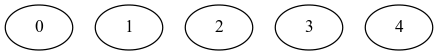
\includegraphics[width=\linewidth]{"./output/graph_prim_iteration_1.png"}

\endminipage\hfill
\minipage{0.20\textwidth}
  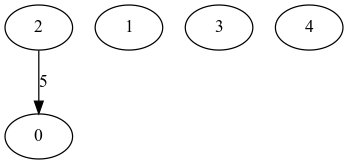
\includegraphics[width=\linewidth]{"./output/graph_prim_iteration_2.png"}

\endminipage\hfill
\minipage{0.20\textwidth}
  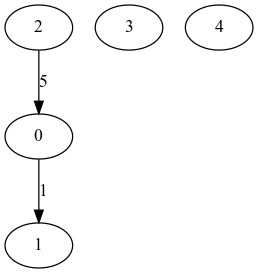
\includegraphics[width=\linewidth]{"./output/graph_prim_iteration_3.png"}

\endminipage\hfill
\minipage{0.20\textwidth}
  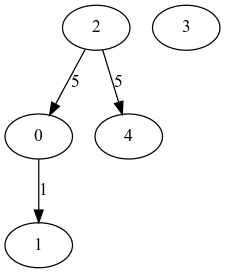
\includegraphics[width=\linewidth]{"./output/graph_prim_iteration_4.png"}

\endminipage\hfill
\minipage{0.20\textwidth}
  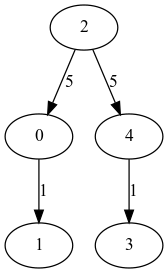
\includegraphics[width=\linewidth]{"./output/graph_prim_iteration_5.png"}

\endminipage
\end{figure}


\newpage
\subsection{Strongly Connected Components}
Ecco un esempio di funzionamento: in ordine, grafo iniziale, grafo inverso, grafo SCCs.

\begin{figure}[!htb]
\minipage{0.32\textwidth}
  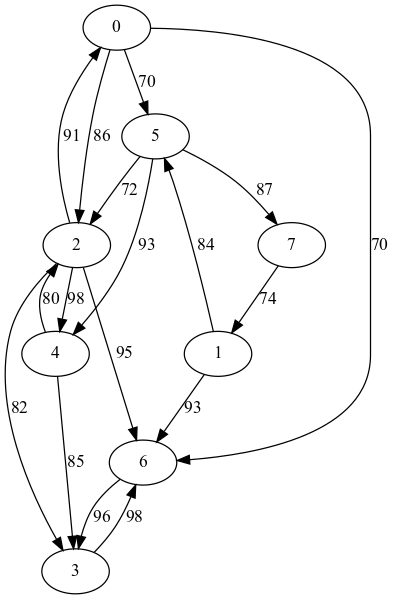
\includegraphics[width=\linewidth]{"./output/scc_example.png"}
  \caption{Original Graph}
\endminipage\hfill
\minipage{0.32\textwidth}
  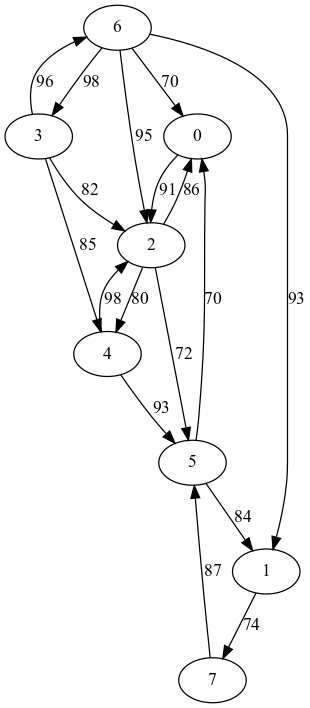
\includegraphics[width=\linewidth]{"./output/scc_example_inv.png"}
  \caption{Inverted Graph}
\endminipage\hfill
\minipage{0.32\textwidth}
  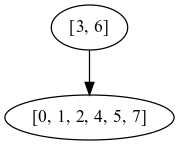
\includegraphics[width=\linewidth]{"./output/scc_example_result.png"}
  \caption{Result}
\endminipage
\end{figure}

I risultati in questo caso sono differenti dalle aspettative, in quanto in media, per grafi grandi si ha solo una SCC. Questo probabilmente accade perchè dato che gli archi sono assegnati casualmente, al crescere del numero dei nodi cresce anche il numero degli archi, con maggiori probabilità di unire più SCCs.
\begin{figure}[!h]
\centering
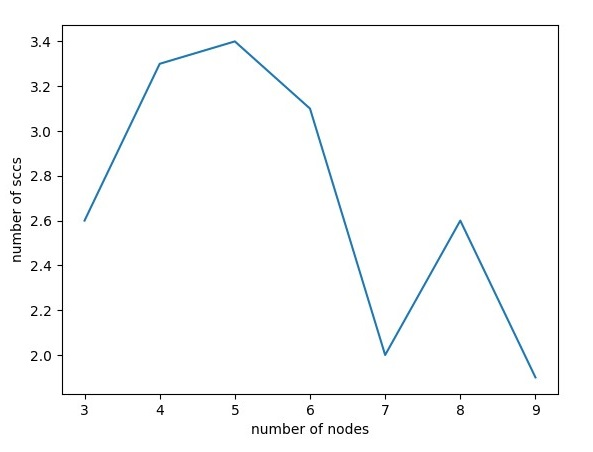
\includegraphics[width=0.45\linewidth]
{"./sccs_to_nodes.jpg"}
\label{graph}
\end{figure}
\end{document}